\section{The Cube Structure}
In this implementation we use an object-orientated approach to the problem.
The \rubik{} is divided into its sub structures which consist of six faces each with nine shared \cubicle{}s each containing a \cubie{}.
There are three types of \cpiece{}s and \cubicle{}s: corners, edges, and centers. 
The \cubie{}s either consist of one, two, or three facelets.
On figure \ref{fig:cubeClassDiagram} the cube class diagram is shown and a detailed description of the classes will explained in the following subsections.
%The cube consist of the 6 faces each with 9 shared \cpiece{}. 

\begin{figure}[htbp]
	\centering
		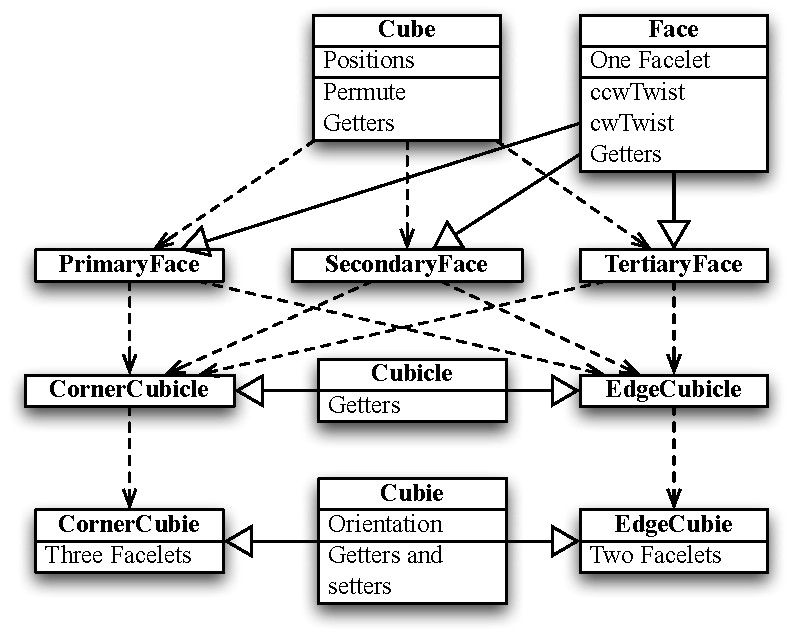
\includegraphics[scale=0.75]{input/pics/cubeClassDiagram.pdf}
	\caption{\myCaption{Class diagram of the cube with properties and methods.}}
	\label{fig:cubeClassDiagram}
\end{figure}

\subsection{The Cube}
The cube class creates 20 \cubicle{}s in which the \cpiece{}s can be positioned. Furthermore the cube class creates the \face{}s and \cubie{}s. Even though the cube class initializes all objects, this is not drawn on the class diagram (see figure \ref{fig:cubeClassDiagram}) because they are not used this way. The cube class also gives each \cpiece{} its \facelet{}s. The \cubicle{}s are then put into a \face{} by its constructor. The cube class creates six \face{}s -- two primary, two secondary, and two tertiary faces. Each type of \face{}s are placed opposite to each other. E.g. the up and down faces are both primary. 

The cube has a static method, \vr{permute}, it recieves two arguments, a cube object and a sequence of \twist{}s. The \twist{} sequence is defined by the same class as the buttons in the GUI, namely the \vr{MoveButtons} class. The moves are named by the Singmaster notation \cite[p. 7]{Joyner02}  where the prime (\m{'}) is replaces by a ``P'', e.g. \m{U'} is \m{UP}.




\subsection{The Face}
\label{sub:cubeFaces}
A face consists of nine \cubicle{}s which act as placeholders for the \cpiece{}s. The center \cpiece{}s will never move and therefore there is no reason to define a \cubicle{} and a \cpiece{} for those. Instead the center piece of a face is granted a \facelet{}, which defines the color of the face in the completed state of the \rubik{}.
The \face{} class constructor takes eight cubicles (four corners and four edges) and positions them in a clockwise order. In addition the \face{} class implements two methods which twist the face clockwise or counterclockwise -- namely \textit{cwTwist} and \textit{ccwTwist} respectively.

There are three different types of \face{}s; primary \face{}s, secondary \face{}s, and tertiary \face{}s, which are defined by their center \facelet{}.
Each type has its own subclass, which inherits from the \face{} superclass.
The reason for the different classes is that there is a difference in how the orientation of the \cubie{}s change depending on what type of \face{} being \twist{}ed.

Each face is known by its type and a number 0 or 1 (see figure \ref{fig:faceRanking}) e.g. the up face is know in the program as \vr{PRIMARY\_0}.
Its opposite is know as \vr{PRIMARY\_1}. 

\begin{figure}[htbp]
	\centering
		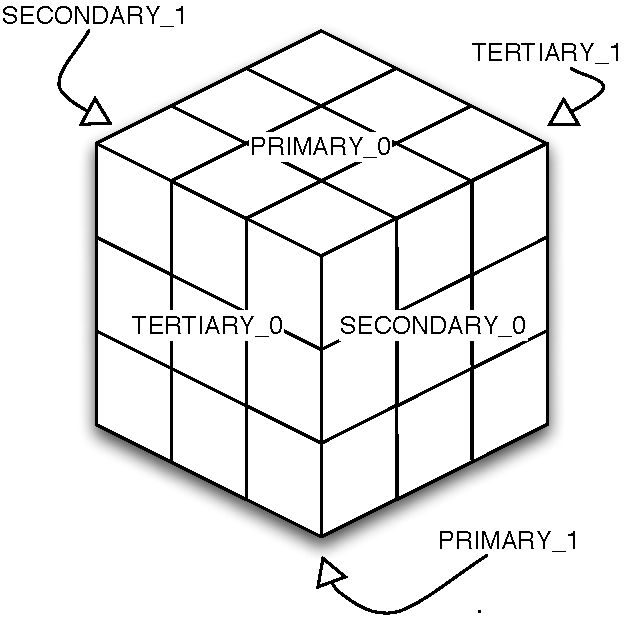
\includegraphics[scale=0.5]{input/pics/faceRanking.pdf}
	\caption{\myCaption{The different faces of a Rubik's Cube. The colors can be defined as whatever one wants.}}
	\label{fig:faceRanking}
\end{figure}

\subsection{The Cubicle}
The \cubicle{} class is a superclass and there are two subclasses to this class; corner- and edge \cubicle{}.
The corner and edge \cubicle{} classes each have one instance variable, namely the \cubie{} they hold. The \cpiece{} is set by the constructor of the \cubicle{} class. 
The \cubie{} can be replaced with another \cubie{} with a setter. 

The different positions are defined by the faces. There are two types of positions; corners and edges.
An edge \cubicle{} could be named \vr{P1S0}; which means \vr{PRIMARY\_1} and \vr{SECONDARY\_0}.  See figure \ref{fig:faceRanking}.

The corner to the right of \vr{P1S0} would be \vr{P1S0T1}, which refers to the corner on the \vr{PRIMARY\_1}, \vr{SECONDARY\_0}, and \vr{TERTIARY\_1} faces. See figure \ref{fig:faceRanking}.


\subsection{The Cubie}
The \cpiece{} class sets the orientation (see section \ref{sec:orientation}) correctly by default, because the cube is assembled correctly when initialized. 
It implements methods that return the orientation and \facelet{}s of the \cpiece{}. 
The \cubie{} class is a superclass and there are two subclasses to this; corner- and edge \cubie{}. 
The corner \cubie{}s contain three \facelet{}s, where edge \cubie{}s only contain two \facelet{}s.
The corner and edge \cpiece{} classes implements two different methods, which return the orientation of the \cpiece{}. 



\subsection{The Facelet}
%%The \facelet{} class is an enumeration that contains the colors of the \facelet{}s, it implements a \textit{toColor} method which define the color of each \facelet{}.
The \facelet{}s are defined in an enumeration which contains the colors of the \facelet{}s, it implements a \textit{toColor} method which define the actual color of each \facelet{}.
The \facelet{}s are divided into primary, secondary, and tertiary \facelet{}s -- 
each consisting of the \facelet{}s of two opposite faces. 